 % -*- coding: utf-8 -*-
% !TEX encoding = UTF-8 Unicode
% !TEX root =  main.tex

\chapter{Theoretische und begriffliche Grundlagen}\label{cha:grundlagen}

Um auf die Regelung einer anisotropen Synchronmaschine einzugehen, werden im Folgendem einige Grundlagen erörtert.

\section{Maxwellsche Gleichungen}\label{sec:maxwell}

Die Grundlage für alle Betrachtungen sind die Maxwellschen Gleichungen.
In Differentialform lauten diese (unter Vernachlässigung des Verschiebungsstromes $\vec{D}$

\begin{tabular}{ll}
1. Maxwellsche Gleichung	&	$\nabla \times \vec{H} = \vec{J}+\frac{\i{d}\vec{D}}{\i{d}t} \approx \vec{J}$ \\
2. Maxwellsche Gleichung	&	$\nabla \times \vec{E} = -\frac{\i{d}\vec{B}}{\i{d}t}$ \\
3. Maxwellsche Gleichung	&	$\nabla \cdot \vec{B} = 0$ \\
4. Maxwellsche Gleichung	&	$\nabla \cdot \vec{D} = \rho$
\end{tabular}

und die dazu gehörigen Materialgesetze lauten

\begin{align*}
\vec{B} &= \mu\vec{H}\\
\vec{D}	&= \epsilon\vec{E}\\
\vec{J} &= \gamma\vec{E}
\end{align*}

Bei homogenen, isotropen Materialien reduzieren sich die Skalarfelder $\mu, \epsilon$ und $\gamma$ zu ortsunabhängigen Materialkonstanten.

\subsubsection{Das Durchflutungsgesetz (1. Maxwellsche Gleichung in Integralfrom)}

\begin{minipage}{0.5\textwidth}
	\begin{align}
		\oint \vec{H}\i{d}\vec{l} = \int_A \vec{J}\i{d}\vec{A}
	\end{align}
\end{minipage}
\begin{minipage}{0.5\textwidth}
	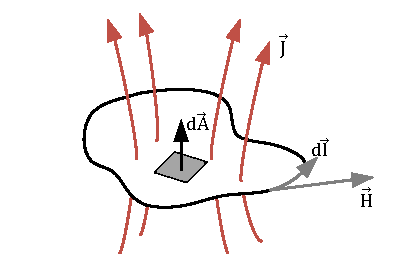
\includegraphics{Gerling1}
\end{minipage}

Das Linienintegral der magnetischen Feldstärke $\vec{H}$ längs eines in sich geschlossenen räumlichen Integrationsweges $\vec{l}$ ist gleich dem gesamten elektrischen Strom, der durch die so begrenzte Fläche $A$ hindurchtritt.

\subsubsection{Das Induktionsgesetz (2. Maxwellsche Gleichung in Integralfrom)}

\begin{minipage}{0.5\textwidth}
\begin{align}
	\oint \vec{E}\i{d}\vec{l} = -\frac{\i{d}}{\i{d}t}\int_A \vec{B}\i{d}\vec{A}
\end{align}
\end{minipage}
\begin{minipage}{0.5\textwidth}
	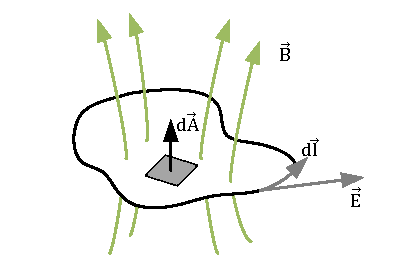
\includegraphics{Gerling2}
\end{minipage}


Das Linienintegral der elektrischen Feldstärke $\vec{E}$ längs eines in sich geschlossenen Integrationsweges $\vec{l}$ ist gleich der negativen totalen zeitlichen Änderung des gesamten magnetischen Flusses, der durch die so begrenzte Fläche A hindurchtritt.

Hierbei ist

\begin{align}
\int_A \vec{B}\i{d}\vec{A} = \Phi
\end{align}

der magnetische Fluss.

\subsubsection{(3. Maxwellsche Gleichung in Integralfrom)}

\begin{align}
\int_A \vec{B}\i{d}\vec{A} = 0
\end{align}

\subsubsection{(4. Maxwellsche Gleichung in Integralfrom)}

\begin{align}
\int_A \vec{D}\i{d}\vec{A} = \int_V\rho\i{d}V
\end{align}

\section{Mehrphasensysteme}
\label{subsec:mehrphasensysteme}

Bei einpoliger Verbindung von $m$ Wechselspannungsquellen entsteht eine Schaltung, die $(m+1)$ Klemmen aufweist (s.~h.~Abbildung~\ref{fig:mehrphasen}).
Haben diese $m$ Wechselspannungsquellen dieselbe Kreisfrequenz $\omega$, so stellt die Schaltung die Spannungsquelle eines allgemeinen Mehrphasensystems dar.

\begin{figure}[!h]
\centering
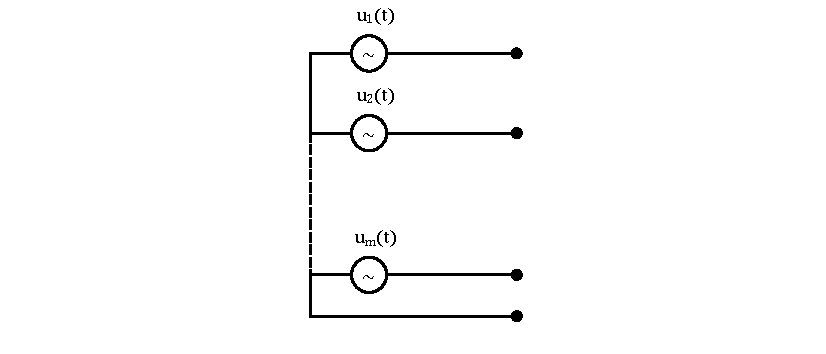
\includegraphics[width=\textwidth]{mehrphasen.pdf}
\label{fig:mehrphasen}
\caption{Spannungsquelle eines Mehrphasensystems.}
\end{figure}

Da keine Vorgaben bezüglich der Amplituden $\hat{u}$ und der Phasenlage $\varphi$ in der Definition der allgemeinen Mehrphasen-Spannungsquelle enthalten sind, kann sie \zB durch das folgende Gleichungssystemen beschrieben werden

\begin{align}
u_\i{1(t)} &= \hat{u}_\i{1} \cdot \cos(\omega t - \varphi_\i{1}) \\
u_\i{2(t)} &= \hat{u}_\i{2} \cdot \cos(\omega t - \varphi_\i{2}) \nonumber  \\
\vdots \nonumber \\
u_\i{m(t)} &= \hat{u}_\i{m} \cdot \cos(\omega t - \varphi_\i{m}) \nonumber
\end{align}

Aus der allgemeinen Mehrphasen-Spannungsquelle entsteht eine symmetrische Mehrphasen-Spannungsquelle, wenn zusätzlich gleiche Amplituden

\begin{align*}
\hat{u}_\i{1} = \hat{u}_\i{2} = \ldots \hat{u}_\i{m}
\end{align*}

und gleiche Phasenwinkeldifferenz zwischen aufeinanderfolgenden Teilspannungen gefordert werden

\begin{align*}
\varphi_\i{1} - \varphi_\i{2} = \varphi_\i{2} - \varphi_\i{3} = \ldots = \varphi_\i{m-1} - \varphi_\i{m} = \Delta \varphi
\end{align*}

Aus Symmetrieüberlegungen ergibt sich, dass die einheitliche Phasenwinkeldifferenz eine Funktion der Phasenzahl $m$ sein muss.

\begin{align}
\Delta \varphi = \frac{\omega T}{m} = \frac{2\pi}{m}
\end{align}

Darin tritt die Periodendauer $T$ der Teilspannungen auf.
Setzt man der Einfachheit

\begin{align*}
\varphi_\i{1} = 0
\end{align*}

so wird die symmetrische Mehrphasen-Spannungsquelle durch das folgende Gleichungssystem beschrieben.

\begin{align}
u_\i{1}(t) &= \hat{u} \cdot \cos(\omega t) \label{eqn:drehstrom} \\ 
u_\i{2}(t) &= \hat{u} \cdot \cos(\omega t - \frac{\omega T}{m})\nonumber \\
\vdots \nonumber \\
u_\i{m}(t) &= \hat{u} \cdot \cos(\omega t - (m-1)\frac{\omega T}{m})\nonumber
\end{align}

In der Elektrotechnik treten Systeme mit verschiedenen Phasenzahlen auf.
Das Wechselstromsystem kann als Sonderfall des Mehrphasensystems mit $m=1$ aufgefasst werden.
Es kommt nur bei kleinen Leistungen zum Einsatz.
Eine Ausnahme stellt die Bahnversorgung dar, die bis zu großen Leistungen generell einphasig betrieben wird.
Gekennzeichnet ist diese durch die eingeprägte Frequenz von $f = 16\frac{2}{3}\mbox{Hz}$.

Die Phasenzahl $m=2$ tritt bei elektrischen Kleinmaschinen auf, allerdings nur in Form eines unsymmetrischen Systems mit einer Phasenwinkeldifferenz

\begin{align*}
\Delta \varphi = 90^{\circ} \,\text{bzw.\ } 270^{\circ}
\end{align*}

Die Phasenzahl $m=3$ kennzeichnet das Drehstromsystem, dass die Basis der elektrischen Energietechnik bildet.
Höhere Phasenzahlen treten \zB in der Stromrichtertechnik auf mit $m=6, 12, 24$.
Drehstromerzeuger mit Phasenzahl $m=3$ werden generell als symmetrisches System ausgelegt.
Als Klemmenbezeichnung ist die Buchstabengruppe $R, S, T$ bzw.\ $U, V, W$ üblich, wobei die gemeinsame Leitung der drei Teilspannungen mit $O, N$ oder $Mp$ für Mittelpunkt bezeichnet wird.

Durch die DIN-Normung wurde festgelegt, dass die Klemmenbezeichnung beim Drehstromsystem mit $L1, L2$ und $L3$ zu erfolgen hat.
Die Phasenwinkeldifferenz ist $\Delta \varphi = 120^{\circ}$.
Stellt man die Phasenspannungen $u_\i{1}(t), u_\i{2}(t), u_\i{3}(t)$ nach Abbildung~\ref{eqn:drehstrom} dar, so ergibt sich 

\begin{figure}[!h]
\centering
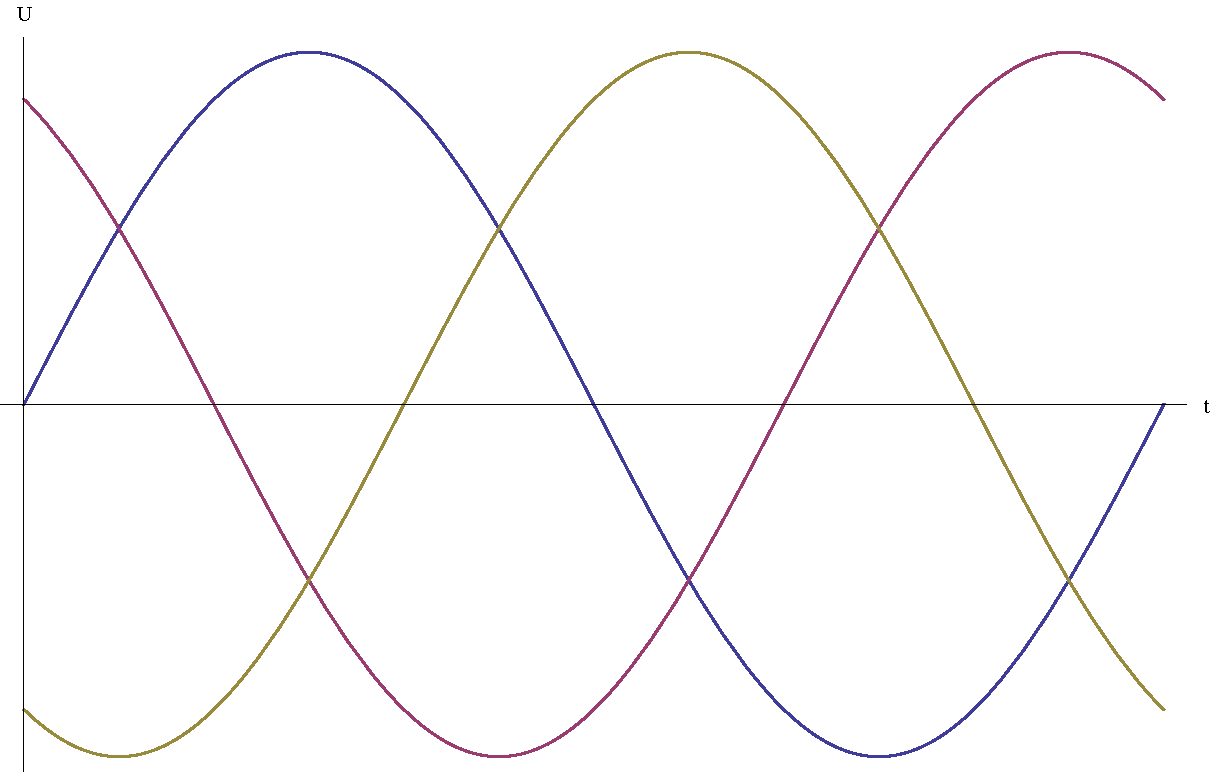
\includegraphics[width=\textwidth]{dreiphasensystem.pdf}
\label{fig:dreiphasen}
\caption{Phasenspannung eines symmetrischen Drehstromerzeugers.}
\end{figure}

\section{Theorie der Drehfeldmaschinen}\label{sec:grund-drehfeld}

Drehfeldmaschinen sind die am häufigsten eingesetzten Antriebsmaschinen, der Grund hierfür ist die Robustheit der aktiven Bauteile und die gute Energieeffizienz.
Zudem besitzen Drehfeldmaschinen ein großes Leistungsspektrum und einen großen Drehzahl- und Drehmomentstellbereich.
Die wesentlichen Vertreter der Maschinenfamilie sind die Synchron- und die Asynchronmaschinen.
Beide basieren auf der Wirkung eines Drehfeldes, das sich durch den Luftspalt der Maschine bewegt.
Die Synchron- und Asynchronmaschine besitzen im Ständer denselben Aufbau und erfordern zur Darstellung ihres Verhaltens eine Reihe gleicher physikalischer Begriffe.
Es ist zweckmäßig die Grundlagen der Synchronmaschine in einem eigenen Kapitel zu behandeln.
Dies gilt \insb für den Aufbau der Drehstromwicklungen sowie die Grundlagen zur Beschreibung von umlaufenden Durchflutungen und deren Felder.

Der prinzipielle Aufbau einer Drehstromwicklung lässt sich anhand aus den Anforderungen zur Erzeugung einer dreiphasigen Wechselspannung erläutern.
Eine solche Drehspannung erhält man mit einer Anordnung nach Abbildung~\ref{fig:drehstromwicklung}.
Ein aus Dynamoblechen geschichtetes Ständerblechpacket enthält in Nuten am Bohrungsumfang gleichmäßig verteilte Leiter, die zu drei räumlich verteilten Wicklungssträngen zusammengeschaltet werden \autocite[S.~141]{fischer2009}.
Der Läufer erzeugt ein Gleichfeld, das eine sinusförmige Feldverteilung längst des Luftspaltes aufbaut.
Hat der Läufer eine konstante Drehzahl, so induziert das Feld in den einzelnen Spulen zeitlich sinusförmige Spannungen, die sich innerhalb eines Wicklungsstranges zu einem Wert addieren.

\section{Magnetfelder}

\subsection{Strombelag}

Das Luftspaltfeld hat die zentrale Bedeutung und muss deshalb auch berechnet werden können.
Die Ursache für die Entstehung dieses Luftspaltfeldes sind die vom Strom durchflossenen Leiter in den Nuten des Stators.
Unter der idealisierten Annahme eines homogenen Feldverlaufs im Bereich der Nutöffnung (s.~h.~Abbildung~\ref{fig:nutquerfeld}) das Feld im Luftspalt vom Feld in der Nut getrennt.

\begin{figure}[!htb]
\centering
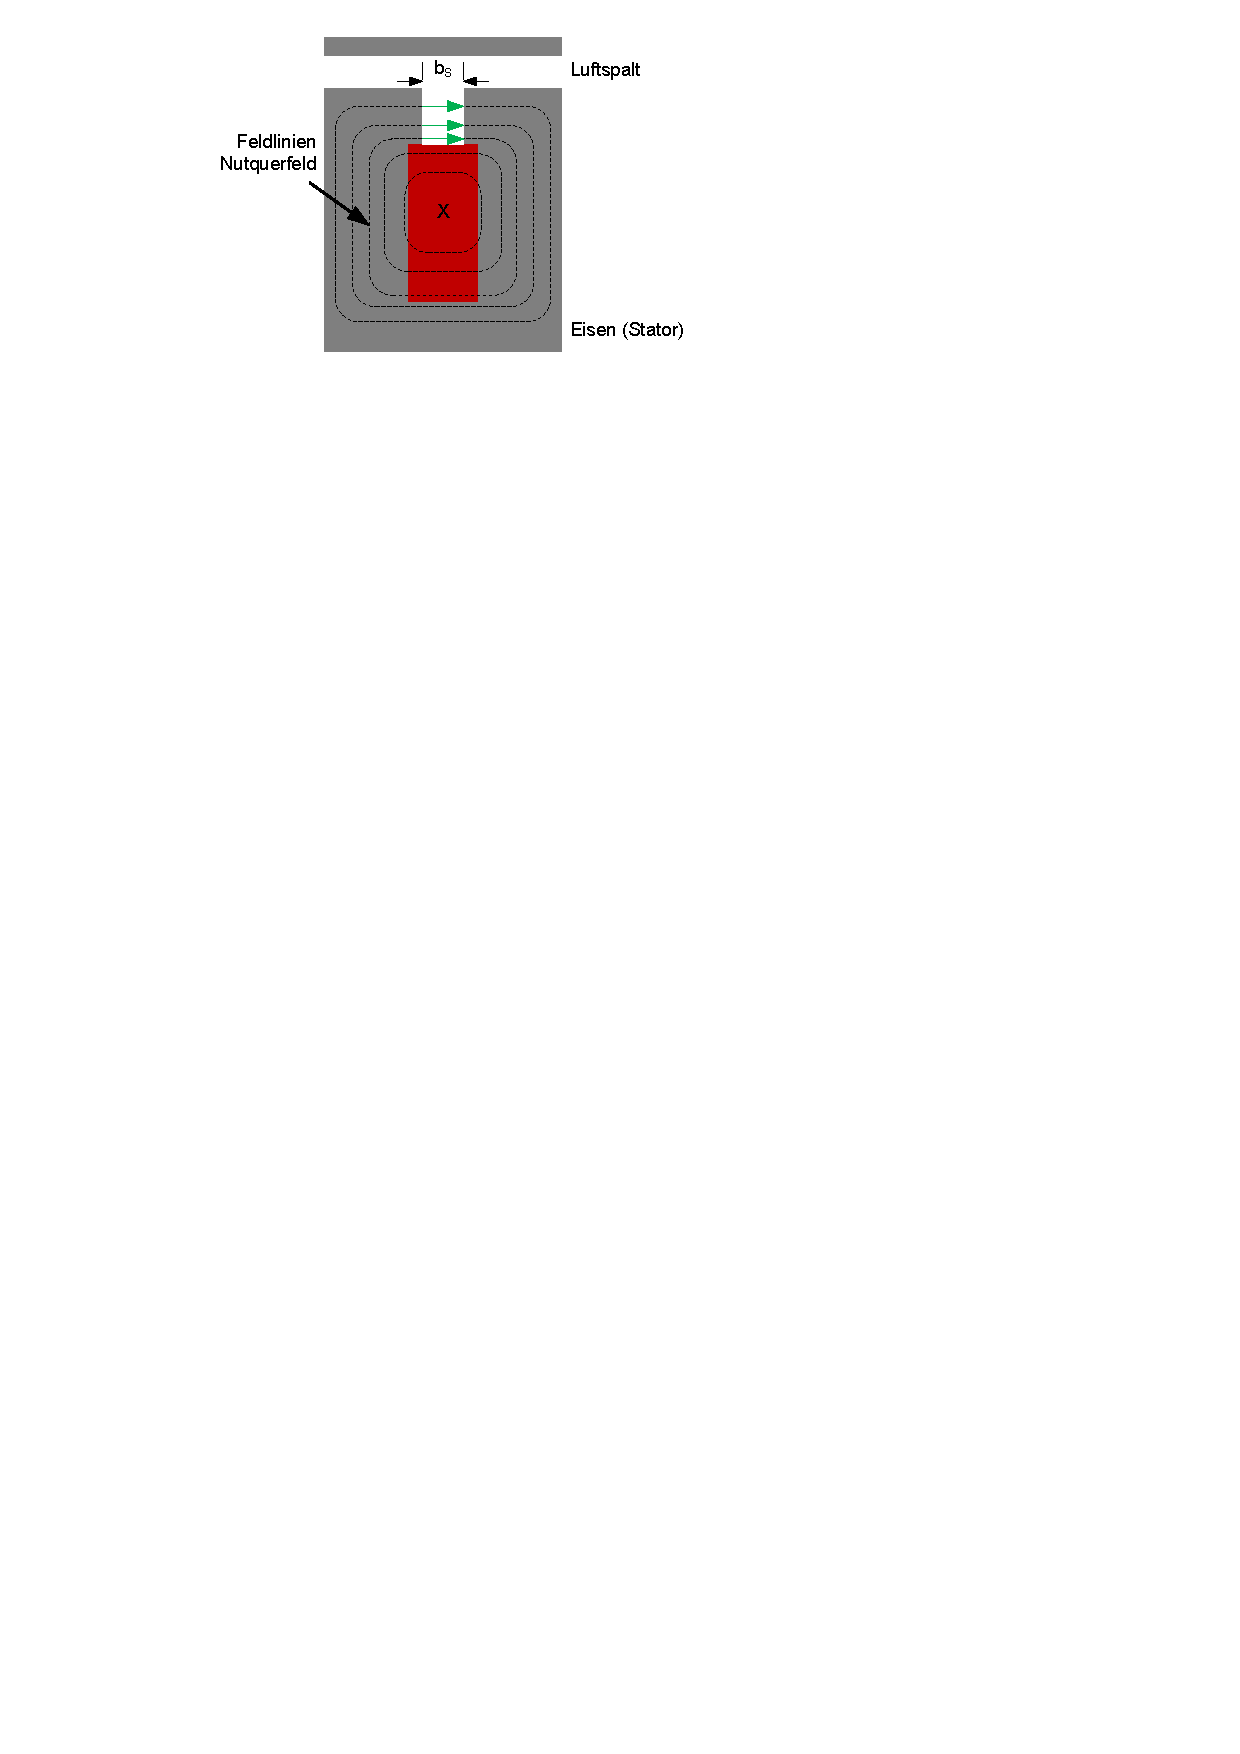
\includegraphics{_Bilder/nutquerfeld.pdf}
\label{fig:nutquerfeld}
\caption{Abbildung des Nutquerfeldes einer Rechtecknut im Stator.}
\end{figure}

Hierzu wird die oben abgebildete Nut betrachtet, wobei die Permeabilität des Eisens als sehr groß gegenüber derjenigen von Luft angenommen wird ($\mu_\i{Fe} \rightarrow \infty$).
Es bildet sich ein Nutquerfeld aus, das ist leicht aus dem Durchflutungsgesetzt herzuleiten.

\begin{align}
\oint \vec{H}d\vec{l} = \Theta \label{eqn:durchflutungsgesetzt}
\end{align}

Dieses Nutquerfeld stößt an der Grenzfläche zwischen Nutöffnung (Nutschlitz bzw.\ Streuschlitz) und Luftspalt an das zu berechnende Luftspaltfeld und stellt somit eine der Randbedingungen zur Berechnung des Luftspaltfeldes dar.
Das Magnetische Feld in der Nutöffnung $H_\i{S}$, dass unter idealisierte Annahme tangential gerichtet ist, kann wiederum auch aus dem Durchflutungsgesetz berechnet werden.

\begin{align}
H_\i{S} = \frac{\Theta_\i{Nut}}{b_\i{S}}
\end{align}

Diese Randbedingung zur Berechnung des Luftspaltfeldes kann auch anders erzeugt werden.
Unter Annahme, dass die Nutdurchflutung $\Theta$ unendlich dünn auf einer glatten Eisenoberfläche gleichmäßig im Bereich der Nutöffnung $b_\i{S}$ verteilt ist.
Diese Modellvorstellung wird mit Hilfe des Strombelages beschrieben.

\begin{align}
A = \frac{\Theta_\i{Nut}}{b_\i{S}}
\end{align}

s.~h.~Abbildung~\ref{fig:strombelag-neu} zeigt die Modellvorstellung der obigen Beschreibung.

\begin{figure}[!h]
\centering
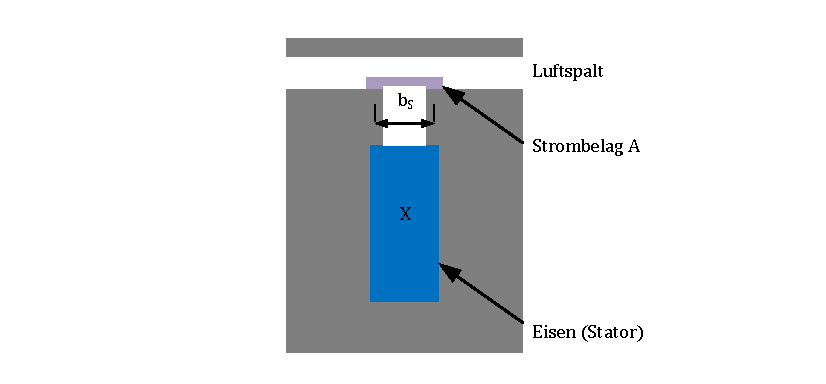
\includegraphics[width=\textwidth]{strombelag_neu.pdf}
\label{fig:strombelag-neu}
\caption{Vereinfachte Modellvorstellung zur Berechnung des Luftspaltfeldes mit Hilfe des Strombelags.}
\end{figure}

Bei Auswertung des Durchflutungsgesetz bei einem Umlauf um diesen Strombelag, ergibt sich für die tangentiale Feldstärke $H_\i{t}$ an der Eisenoberfläche im Bereich des Strombelages

\begin{align}
\oint \vec{H}d\vec{l} = \Theta_\i{Nut} \\
H_\i{t}\cdot b_\i{S} = A\cdot b_\i{S} \\
H_\i{t} = A = \frac{\Theta_\i{Nut}}{b_\i{S}} \label{eqn:feld-ht}
\end{align}

Mit Abbildung~\ref{eqn:feld-ht} ist gezeigt, dass die Randbedingungen zur Berechnung des Luftspaltfeldes unverändert erhalten bleibt, wenn statt der in Nuten eingebrachten Leiter ein äquivalenter Strombelag auf der glatten Eisenoberfläche berücksichtigt wird (Die Wirkung der Nutdurchflutung wird hinreichend genau durch den über der Nutöffnung verteilten Strombelag beschrieben).
Zur Berechnung des Luftspaltfeldes muss also nun das Nutenfeld nicht berücksichtigt werden.
Zudem kann eine deutlich vereinfachte Geometrie zugrunde gelegt werden.

\begin{quote}
\enquote{Die Begrenzungsflächen von Stator und Rotor können als glatt angenommen werden, was in Umfangsrichtung der Maschine konstanten Luftspalt und demzufolge auch einen kostanten magnetischen Luftspaltleitwert entspricht. (Gerling 2008, \emph{Elektrische Maschinen und Antriebe}. Bundeswehr Universität in München.)}
\end{quote}

\paragraph{Weitere spezifische Darstellungen zum Strombelag.}
Die räumliche Verteilung des Stromes wird durch den Strombelag wiedergegeben, der als Leiterzahl $\times$ Stromstärke pro Länge des stromdurchflossenen Umfanges bei rotatorischen Maschinen als \autocite[S.~199]{hofmann2013}

\begin{align}
A = \frac{I \cdot w}{x_\i{S}\cdot p} = \frac{2m \cdot Z\cdot I}{\pi \cdot d_\i{i}} \label{eqn:strombelag2}
\end{align}

betrachtet man jetzt die Polteilung $\tau_\i{p}$

\begin{align}
\tau_\i{p} = \frac{\pi \cdot d_\i{i}}{2p} \label{eqn:polteilung}
\end{align}

so wird aus Gleichung~\ref{eqn:strombelag2} und Gleichung~\ref{eqn:polteilung} bei voller Bewicklung über eine Polteilung

\begin{align}
A = \frac{m w I}{p \tau_\i{p}}
\end{align}

\begin{quote}
\enquote{Aus dem Strombelag $A$ wir bei rotatorischen Maschinen abhängig von der Umfangskoordinate mit $A(x)$, wenn:
\begin{itemize}
\item sich durch Wechsel von Hin- und Rückleiter einer Wicklung die Stromrichtung ändert,
\item durch Konzentration der Wicklung der Strom in den Lücken zu Null wird.
\end{itemize}
\autocite[S.~199]{hofmann2013}}
\end{quote}

Der alternierende Strombelag $A$ kann mit Hilfe der Fourier-Reihenentwicklung durch seine Grundwelle beschrieben werden

\begin{align}
A_\i{1}(x) = \hat{A}_\i{1} \cdot \cos(\frac{x}{\tau_\i{p}}\cdot \pi)
\end{align}

Die wichtigste Kenngröße zur Erzeugung der Kräfte in Maschinen sind die Feldgrößen, d.\ h.\ bei Vernachlässigung des magnetischen Spannungsabfalls im Eisen kann laut dem Durchflutungsgesetz mit $\mu_\i{Fe} >> 1$ die magnetische Spannung über den Luftspalt an jeder Stelle der Umfangskoordinate $x$ über das Integral des Strombelages ermitteln (s.~h.~Abbildung~\ref{fig:Visio-strombelag-hofmann}).

\begin{align}
V_\delta (x) = - \int_0^x A(x)\i{d}x
\end{align}

Das Integral erhält die Bezeichnung \enquote{Felderregerkurve} (vgl.~\textcite[S.~199]{hofmann2013}).
Die Felderregerkurve gibt an, welche magnetische Spannung zur Magnetfelderzeugung an der Stelle $x$ zur Verfügung steht.
Diese ist wichtige für die Berechnung von Streuungs- und Verlusteffekten in der Maschine.

\subsection{Durchflutung}\label{sec:durchflutung}

Die Durchflutung lässt sich als Integral des Strombelages entlang der Polteilung darstellen

\begin{align}
\Theta = -\int_0^{\tau_\i{p}} A(x)\i{d}x
\end{align}

mit Gl.~\ref{eqn:polteilung} ergibt sich nach \textcite[S.~200]{hofmann2013}

\begin{align}
\Theta = - \int_0^{2(\pi /p)} A(\gamma)\i{d}\gamma \quad \text{mit}\,\, \frac{x}{\tau_\i{p}}=\frac{\gamma}{\pi}
\end{align}

\subsection{Gleichfelder}\label{sec:gleichfelder}

Wird der Strombelag einer Wicklung durch einen Gleichstrom gebildet, so entsteht ein örtlich, nicht zeitlich abhängiges Luftspaltfeld.
Die örtliche Abhängigkeit hängt von den Wicklungsparametern ab.
Abbildung~\ref{fig:Visio-strombelag-hofmann} zeigt Strombelag $A$ und Felderregerkurve $B$ einer Vollpol-Ankerspule.
Der Strombelag ist konzentriert, die Felderregerkurve wird trapezförmig an den Sinus angenähert.
Der Induktionsverlauf lässt sich allgemein nach Fourier-Reihenentwicklung durch die Grundwelle beschreiben

\begin{align}
B_\i{1}(x) = \hat{B}_\i{1}\cdot\cos(\frac{x}{\tau_\i{p}}\cdot \pi)
\end{align}

\begin{figure}[h!]
\centering
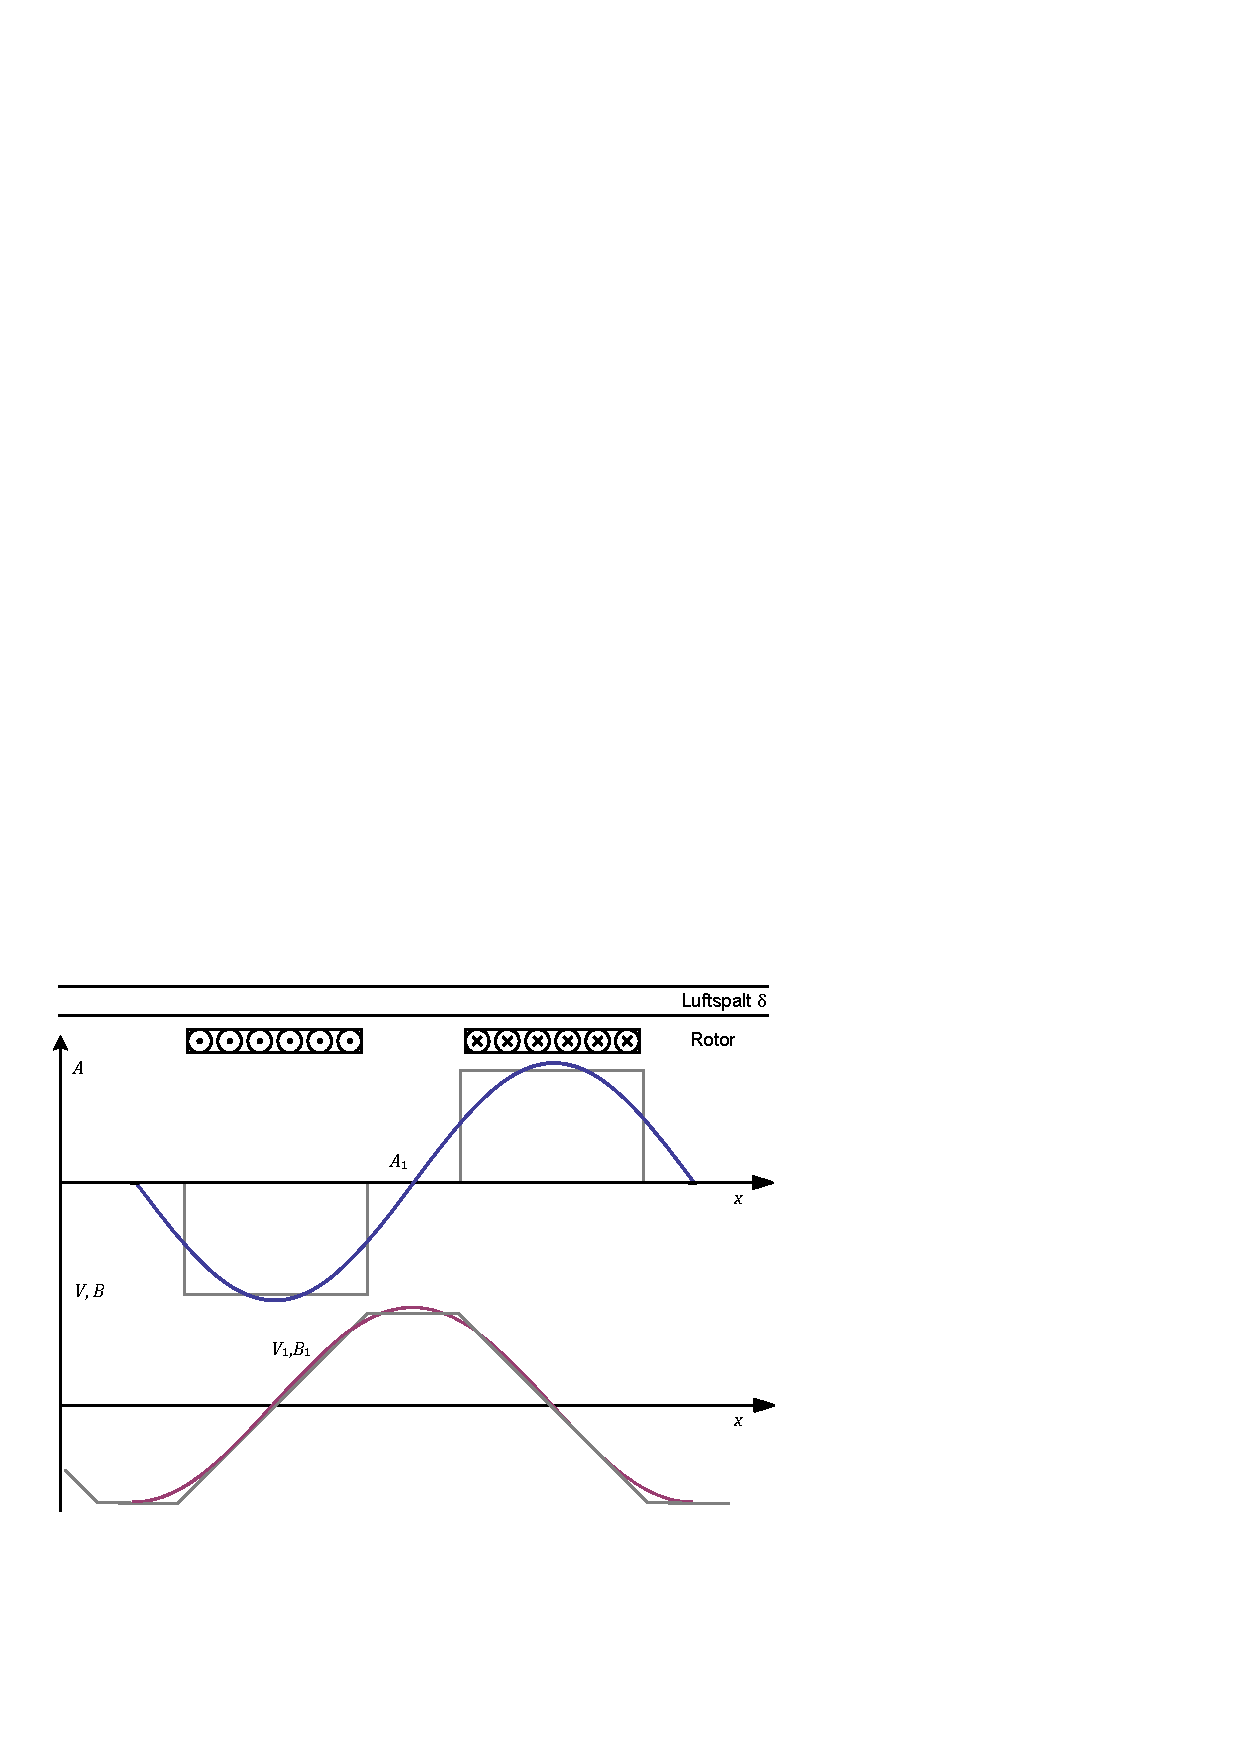
\includegraphics[width=\textwidth]{Visio-strombelag-hofmann.pdf}
\label{fig:Visio-strombelag-hofmann}
\caption{Strombelag, Felderreger- und Feldkurve der Vollpolmaschine.}
\end{figure}

Nutzbare Gleichfelder treten auf als:
\begin{itemize}
	\item Erreger- und Ankerfeld in Gleichstrommaschinen
	\item Erregerfeld in Vollpol-Synchronmaschine
\end{itemize}

\subsection{Drehfelder}\label{sec:drehfelder}

Nach \textcite{hofmann2013} sind Drehfelder

\begin{quote}
\enquote{[\ldots] sind Magnetfelder, deren Welle durch den Luftspalt läuft.}
\end{quote}

Die Erzeugung von Drehfeldern kann auf zwei Arten geschehen.
Zum einen aus der Drehung eines Gleichfeldes (s.~h.~Abschnitt~\ref{sec:gleichfelder}) oder durch die Überlagerung von räumlich verteilten und zeitlich versetzten Wechselfeldern.
Bei der Synchronmaschine wird mittels Gleichstrom der Anker erregt, so entsteht zunächst ein Gleichfeld mit örtlicher Induktionsverteilung.
Wird nun die das Gleichfeld erzeugende Wicklung gedreht, bekommt das Feld eine Drehgeschwindigkeit, d.\ h.\ die Felddichte verhält sich orts- und zeitabhängig.

\begin{align}
B(x,t) = \hat{B}\cdot\cos(\frac{x}{\tau_\i{p}}\pi\pm\omega t)
\end{align}

Der Fall, dass sich aus der Überlagerung von räumlich verteilten und zeitlich versetzten Wechselfeldern ein Drehfeld bildet soll hier nicht weiter erläutert werden.

%\section{Induktivitäten}\label{sec:induktiv}

%Innerhalb der Vektorregelung (s.~h.~Abschnitt~\ref{cha:Grundlagen der Vektorregelung}) werden die absoluten Induktivitäten zum Beispiel für die Berechnung des Spannungssollwertmodells, also der Vorsteuerung, benötigt.
%Im Rahmen von geberlosen Regelalgorithmen sind die absoluten und differentiellen Induktivitäten erforderlich~--~wie \textcite{kellner2012}[S.~35ff.] gut darstellt.
%Auch bei aktuellen Forschungsthemen »Parameteridentifikation von Synchronmaschinen« zeigt \textcite{kellner2012} auf S.~148ff., dass die Induktivitäten für Ständerwiderstandsidentifikation benötigt werden.
%Da für die Anwendung nur die Parameter in rotorfesten Koordinaten von Belang sind, wird sich die Sichtweise in der vorliegenden Arbeit darauf beschränken.

%In den Spannungsgleichungen (s.~h.~Abschnitt~\ref{sec:spannungsgleichung-esb}) der Wicklungen einer elektrischen Maschine sind neben den ohmschen Spannungsabfällen $u$ die zeitlichen Änderungen ihrer Flussverkettungen $\Psi$ \autocite[S.~511]{mullerII2008}.
%Sowohl die Flussverkettung als auch die ohmschen Spannungsabfälle sind Funktionen der Ströme $i$.
%Bei ohmschen Spannungsabfällen tritt als Proportionalitätsfaktor der Wicklungswiderstand $R$ auf.
%Bei magnetischer Linearität zwischen den Strömen und der Flussverkettung ist $L$ der Proportionalitätsfaktor.

%\begin{quote}
%\enquote{Wenn magnetische Linearität vorausgesetzt wird, kann die Flussverkettung einer Wicklung ganz allgemein als Linearkombination ihrer von den %einzelnen für das Feld verantwortlichen Strömen herrührenden Anteile dargestellt werden \autocite[S.~511]{mullerII2008}.} 
%\end{quote}

%Die dort auftretenden Proportionalitätsfaktoren sind Induktivitäten $L$.
%Für die Flussverkettung $\Psi_\i{n}$ einer Wicklung $n$ mit dem gesamten Feld des Stromes $i_\i{k}$ der Wicklung $k$ gilt

%\begin{align}
%\Psi_\i{n} = L_\i{n,k}\cdot i_\i{k} = \int_\i{Wicklung n}B_\i{k}\i{d}A \label{eqn:induktivität}
%\end{align}

%Dabei stellt der Proportionalitätsfaktor $L$ zwischen der Flussverkettung einer Wicklung und ihrem eigenen Strom die Selbstinduktivität dar \autocite[S.~24]{ternes2013}.
%Ströme die in anderen Wicklungen fließen, nennt man Gegeninduktivitäten.
%Ausgehend von Gl.~\ref{eqn:induktivität} ergibt sich die allgemeine Berechnungsvorschrift für eine Induktivität $L_\i{n,k}$ die Beziehung

%\begin{align}
%L_\i{n,k} = \frac{\Psi_\i{n}}{i_\i{k}} \label{eqn:allg-induktivität}
%\end{align}

%Die Induktivitäten lassen sich im stationären Betrieb der Maschine lasssen sich entsprechend Reaktanzen zuordnen.

%\begin{align}
%X = \omega L
%\end{align}

%\subsection{Streuinduktivitäten und Streureaktanzen}\label{sec:induktiv-streu}

%Man erhält die Streuinduktivität gemäß der allgemeinen Beziehung in Gl.~\ref{eqn:allg-induktivität}.
%Das prinzipielle Vorgehen zur Berechnung von Streuflussverkettungen kann aus \textcite[S.~311]{mullerII2008} entnommen werden.
%Entsprechend ergeben sich verschiedene Arten von Streuung.

%\subsubsection{Nut- und Zahnkopfstreuung}\label{sec:nut-zahn-streuung}

%Nach \textcite[S.~323]{mullerII2008} erhält man für die Teilstreufelder im Nut- und Zahnkopfraum entsprechend umgerechnet in die Streureaktanz

%\begin{align}
%X_{\sigma} = \omega L_{\sigma}
%\end{align}

%Nach \textcite[S.~533--536]{mullerII2008} ergibt sich für den allgemeinen relativen Streuleitwert

%\begin{table}[htb]
%\centering
%\caption{Abhängigkeiten für den allgemeinen relativen Streuleitwert nach \textcite{mullerII2008}.}
%\begin{tabular}{ll}
%\toprule
%Streuungskomponente	&	$\lambda_{\sigma} =$ \\
%\midrule
%Nut- und Zahnkopfstreuung	&	$\frac{\lambda_\i{nz}}{q}$ \\
%Wicklungskopfstreuung		&	$\lambda_\i{w}$ \\
%Oberwellenstreuung			&	$\sigma_\i{o}\lambda_\i{h}\xi^{2}_{\i{p}}$	\\
%Schrägungsstreuung			&	$\sigma_\i{schr}\lambda_\i{h}\xi^{2}_{\i{p}}$ \\
%\bottomrule
%\end{tabular}
%\end{table} 

\section{Einführung Synchronmaschine}\label{sec:synchron}

Die ersten Synchronmaschinen wurden als Einphasengenerator entwickelt und gebaut, den ersten dreiphasigen Synchrongenerator entwickelten 1887 unabhängig voneinander F.~A.~Haselwander\footnote{Friedrich August Haselwander war ein deutscher Ingenieur, ein Erfinder der Drehstrom-Synchronmaschine und des kompressorlosen Ölmotors.} und C.~S.~Bradley\footnote{Charles Schenk Bradley war ein US-amerikanischer Elektrotechniker, Erfinder und Pionier von frühen Elektromotoren. Er zählt neben F.~A.~Haselwander zu den Begründern des heute im Bereich der elektrischen Energietechnik eingesetzten Dreiphasenwechselstromes.} Bei den Entwicklungen bildeten sich die Bauformen der Schenkelpol- und Vollpolmaschine aus. Die Weiterentwicklung der Synchronmaschine hing stark mit dem Ausbau der Energieversorgung und dem Bedarf von leistungsstärkeren Generatoren zusammen. Unabhängig von der Entwicklung wurden schon sehr früh Synchronmaschinen als Antriebsmaschinen für eine konstante Drehzahlregelung oder einen Phasenbetrieb in der Industrie eingesetzt \autocites[S.~287]{fischer2009}[S.~485f.]{mullerI2005}.

\begin{figure}[h!]
\centering
\begin{minipage}{6cm}
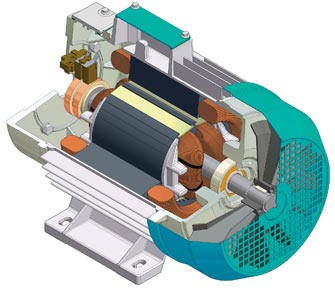
\includegraphics[width=\textwidth]{synchron}
\end{minipage}
\hfill
\begin{minipage}{6cm}
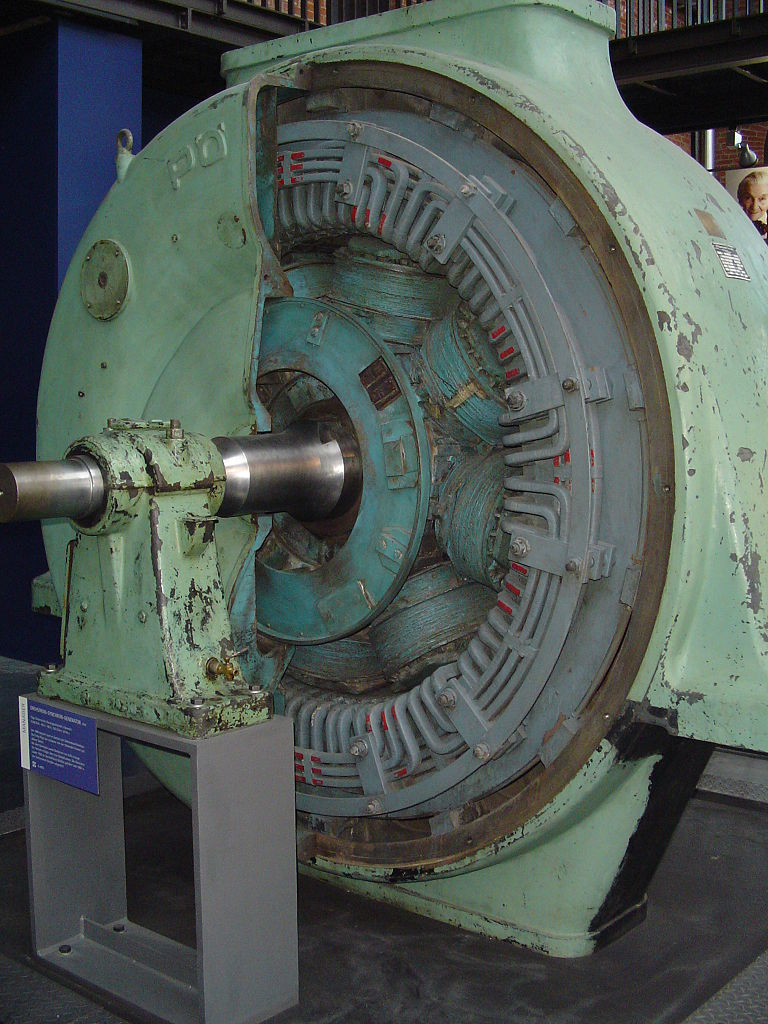
\includegraphics[width=\textwidth]{synchron2}
\end{minipage}
\caption{Abbildungen zweier Synchron Generatoren verschiedener Leistungsklassen.}
\label{fig:synchron-generatoren}
\end{figure}

Die gleichstromgespeiste Erregerwicklung ermöglicht es, das Magnetfeld unabhängig vom Netz zu beeinflussen.
Als Spannungsquelle für die Speisung der Erregerwicklung wurden sog.\ Gleichstromerregermaschinen eingesetzt, in der heutigen Zeit werden Wechselspannung mit Hilfe von Leistungselektronischen Schaltungen gespeist.
Um die Schleifringübertragung der Erregerleistung zu umgehen, werden schleifring- bzw.\ bürstenlose Erregersysteme realisiert \autocite{fischer2009}.
Als Motor wurden Drephasen-Synchronmaschinen schon bald für große Leistungen eingesetzt, \zB zum Antrieb von Pumpen und Verdichten \autocite[S.~486]{mullerI2005}.
Der Nachteil ist, dass die Drehzahl durch die Netzfrequenz festgelegt ist.
Die Synchronmaschine arbeitet unabhängig von der Belastung stets mit der durch die Netzfrequenz und die ausgeführte Polpaarzahl festgelegten synchronen Drehzahl.

Heute ist es möglich, mit Hilfe eines Frequenzumrichters die Drehzahl der Synchronmaschine zu steuern.
Aus diesem Grund werden größere Gleichstrommaschinen durch drehzahlvariable Synchronmaschinen abgelöst.
Im Bereich kleinerer Leistungen wird anstelle der Gleichstromerregung eine Erregung durch Permanentmagnete eingesetzt.
Dabei verliert man die Beeinflussung des Erregerzustandes über den Erregerstrom, dafür erhält man eine elektrische Maschine die keine elektrische Verbindung zum Läufer erfordert.

\subsection{Spannungsgleichungen und Ersatzschaltbild}\label{sec:spannungsgleichung-esb}

Die Synchronmaschine mit Vollpolläufer ist wegen ihres konstanten Luftspaltes mathematisch leichter erfassbar, als die Synchronmaschine mit Schenkelpolläufer.
Als Grundlage für weitere Betrachtungen dient dieses mathematische Modell als Grundlage.
Weiterhin wird vereinbart, dass

\begin{itemize}
	\item quasistationärer Betrieb
	\item Verbraucherzählpfeilsystem
	\item rechtsgängige Spulen
	\item läuferfeste, komplexe Ebene
\end{itemize}

vorliegt s.~h.~Abbildung~\ref{fig:dq-synchron-1}.

\begin{figure}[!h]
\centering
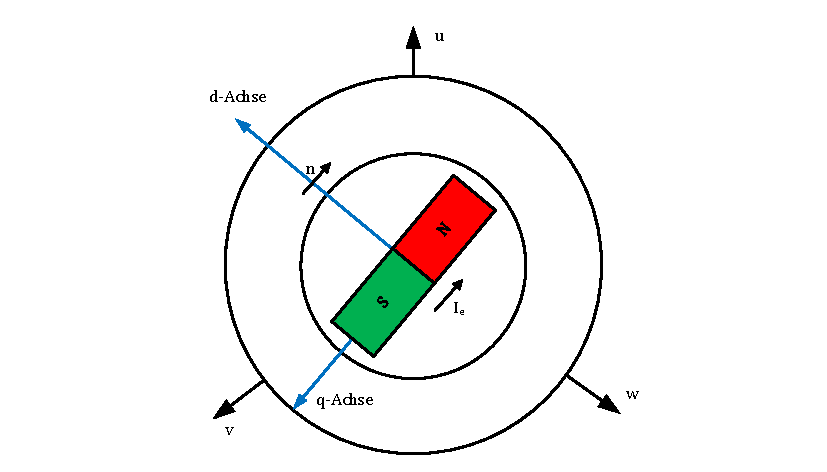
\includegraphics[width=\textwidth]{synchron-dq-1.pdf}
\label{fig:dq-synchron-1}
\caption{Veranschaulicht das mit $n$ rotierende $d, q-$System, in dem der Maschinenzustand durch ruhende Zeiger ausgedrückt wird.}
\end{figure}

Der Ständerkreis kann in den Läuferkreis keine Spannung induzieren, weil Ständerfeld und Läuferfeld gleiche Drehzahl haben und somit im Läufer keine ständerbedingten Flussänderungen entstehen.
Mit dieser Erkenntnis und den oben genannten Voraussetzungen wird der Läuferkreis durch die Gleichung

\begin{align}
U_\i{e} = I_\i{e} \cdot R_\i{e}
\end{align}

beschrieben.

Die Induktivität $L_\i{e}$ bringt wegen

\begin{align*}
\frac{\i{d}i_\i{e}}{\i{d}t} = 0
\end{align*}

keinen Beitrag.
Die Spannungsgleichung für den Ständerkreis ergibt sich zu

\begin{align}
U_\i{1} = R_\i{1}\underline{I}_\i{1}+\i{j}X_\i{1}\underline{I}_\i{1}+\i{j}X_\i{h}\underline{I}_\mu
\end{align}

Bei der Synchronmaschine entsteht die Magnetisierungsstrombelagswelle aus der Ständer- und der Läuferstrombelagswelle.
Der Magnetisierungsstrom setzt sich entsprechend zusammen

\begin{align}
\underline{I}_\mu = \underline{I}_\i{1} + I'_\i{e}
\end{align}

Damit ergibt sich für die Ständerspannung $U_\i{1}$

\begin{align}
U_\i{1} = R_\i{1}\underline{I}_\i{1} + \i{j}X_\i{1}\underline{I}_\i{1} + \i{j}X_\i{h}\underline{I}_\i{1} + \i{j}X_{h}\underline{I}'_\i{e}
\end{align}

Der vom Ständerstrom unabhängige Term wird als eingeprägte Spannung aufgefasst.
Die Polradspannung

\begin{align}
\underline{U}_\i{p} = \i{j}X_\i{h}\underline{I}'_\i{e}
\end{align}

ist über den Erregerstrom einstellbar.
Die Ständerhauptreaktanz $X_\i{h}$ korrespondiert mit dem Drehfeld.
Die Hauptfeldspannung

\begin{align}
\underline{U}_\i{h} = \i{j} X_\i{h} \underline{I}_\i{1} + \underline{U}_\i{p}
\end{align}

hat wie das Drehfeld zwei Komponenten, eine ständerbedingte und eine polradbedingte.

\begin{figure}[!htb]
\centering
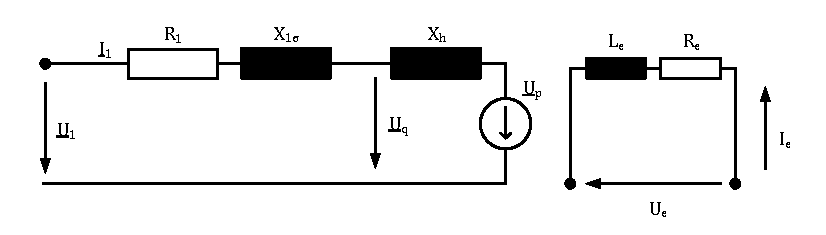
\includegraphics[width=\textwidth]{synchron-esb-kremser2004.pdf}
\label{fig:esb-kremser}
\caption{Ersatzschaltbild der Synchronmaschine.}
\end{figure}

Haupt- und Streureaktanz des Ständerkreises werden häufig zur synchronen Reaktanz zusammengezogen

\begin{align}
X_\i{d} = X_\i{1} + X_\i{h}
\end{align}

Die daraus folgende relative synchron Reaktanz ist eine wichtige Kenngröße der Synchronmaschine.

\begin{align}
x_\i{d} = \frac{I_\i{1}}{U_\i{1}}\cdot X_\i{d}
\end{align}

Als Richtwert gilt

\begin{align*}
x_\i{d} &= 1.2 \ldots 1.5\quad\text{Vollpolläufer} \\
x_\i{d} &= 0.6 \ldots 1.6\quad\text{Schenkelpolläufer}
\end{align*}

Der Ständerkreisverlustwiderstand ist etwa mit 

\begin{align}
R_\i{1} \approx 0.07\cdot X_\i{d}
\end{align}

anzusetzen.

\begin{figure}[!htb]
\centering
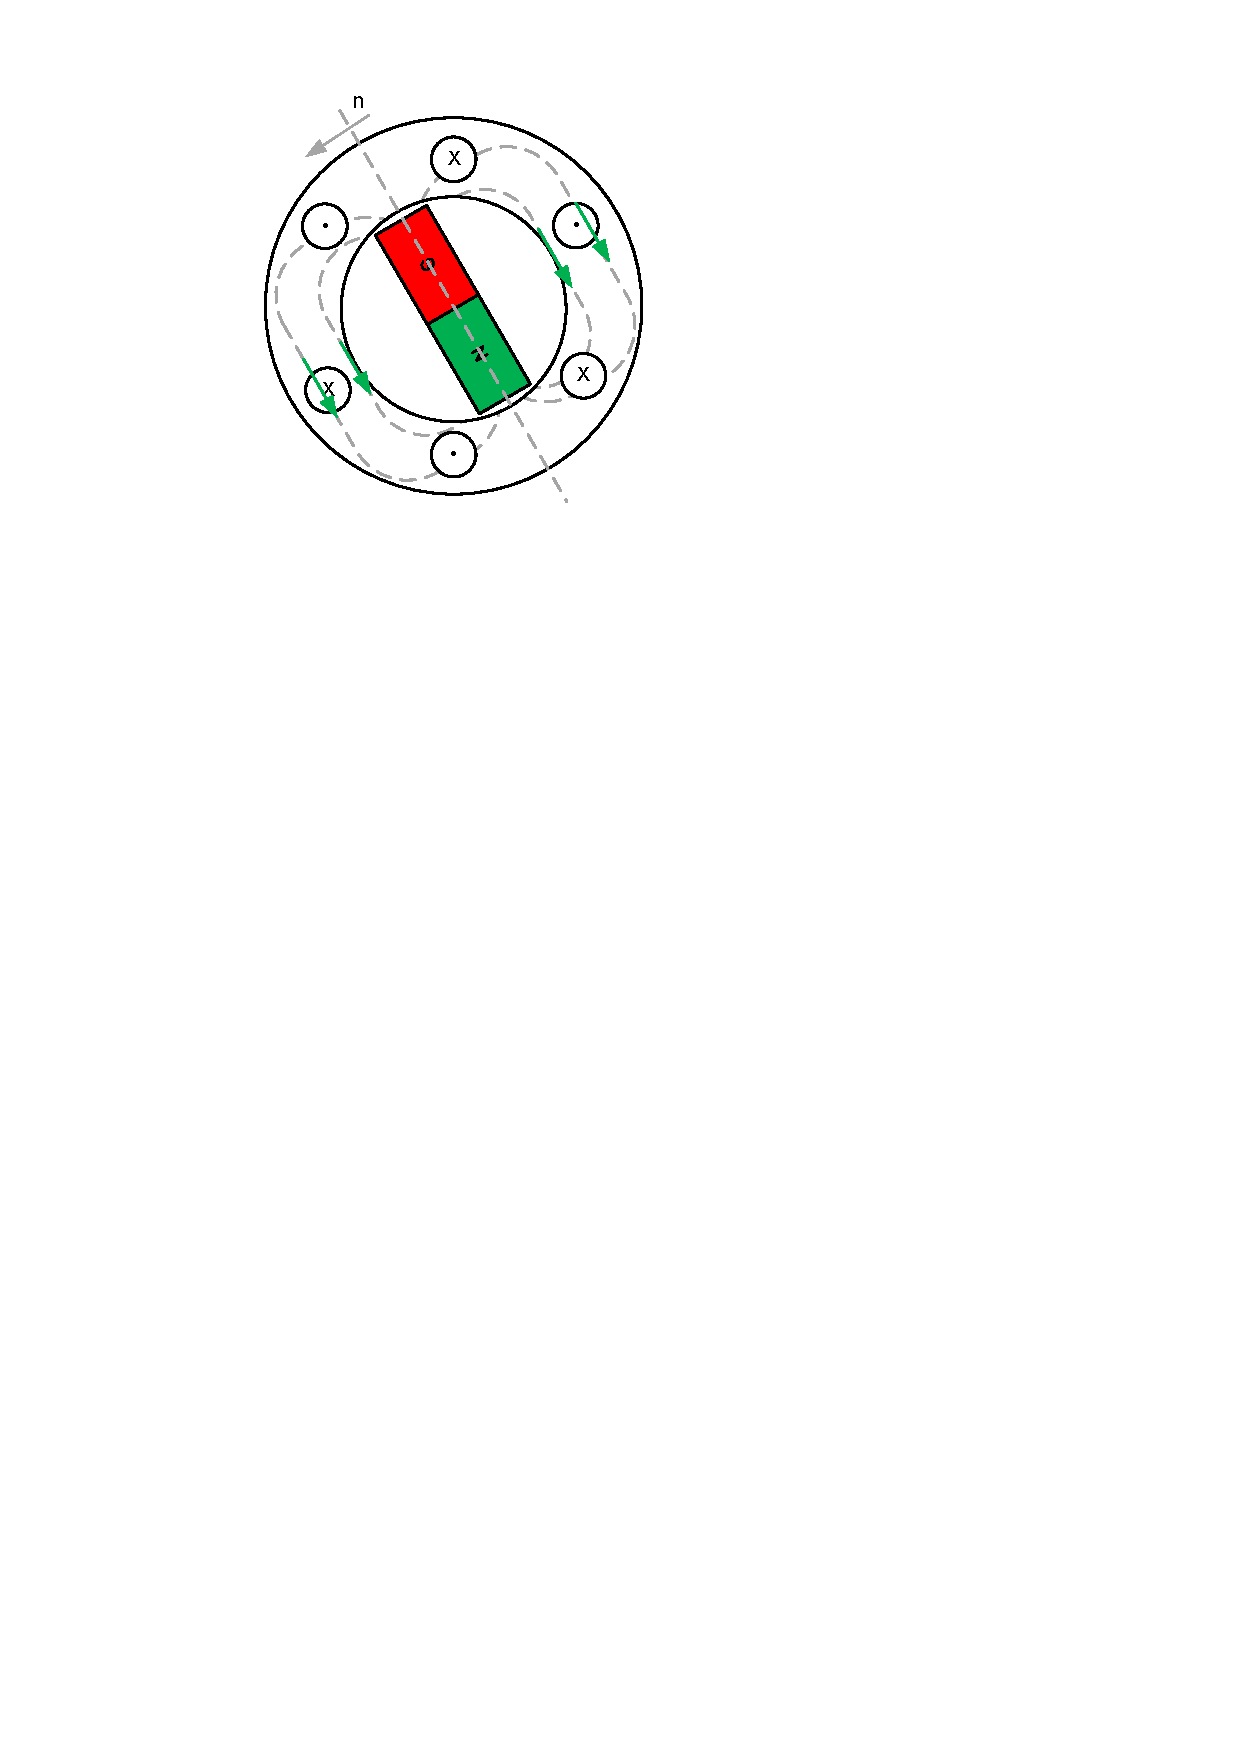
\includegraphics{synchronmaschine-drehstrom.pdf}
\label{fig:drehstromwicklung}
\caption{Erzeugung einer mehrphasigen Spannung durch ein räumlich sinusförmiges Läuferdrehfeld.}
\end{figure}

\subsection{Beschreibung der Synchronmaschine im d,q-Koordinatensystem}\label{sec:synchron-dq}

Im Folgenden wird angenommen, dass die Speisung des Polrads durch Permanentmagnete ersetzt wird.
In diesem Fall verbleiben nur die drei Statorwicklungen als stromdurchflossene Wicklungen.
Wesentlich bei den nachstehenden Überlegungen ist es, ob die Synchronmaschine als symmetrische Maschine (Vollpolläufer) oder als unsymmetrische Maschine (Schenkelpolläufer) konzipiert ist.
Die Wahl der Konzipierung hat Auswirkungen auf die Möglichkeit, Feldschwächebetrieb zu erreichen oder nur bedingt und dann mit Einschränkungen \autocite[S.~291]{schroder2000}.

\begin{figure}[!htb]
\centering
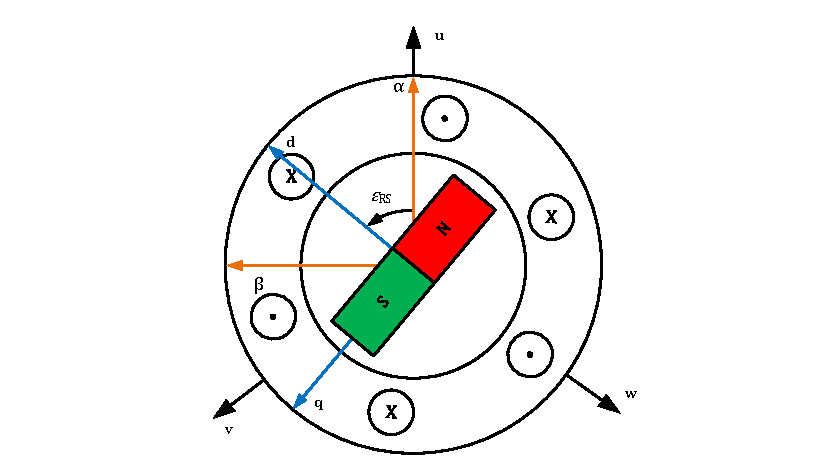
\includegraphics{synchron-dq.pdf}
\label{fig:synchron-dq}
\caption{Darstellung der Synchronmaschine im dq-Koordinatensystem.}
\end{figure}

Wird die Synchronmaschine in der Statorwicklung mit einer sinusförmigen Spannung versorgt, so ist diese als (PMSM) permanentmagneterregte Synchronmaschine definiert.
Bei einer trapezförmigen Speisung der Statorwicklung wird die Maschine als (BLDC) bürstenlose Gleichstrommaschine bezeichnet.
Der einfachste Fall für die Ermittlung des Signalflussplanes ist die Annahme, dass die Maschine an der Statorwicklung eine sinusförmige Spannung anliegt und die Maschine symmetrisch konzipiert wurde.
Bei einer symmetrisch konzipierten Synchronmaschine werden die Reluktanzeinflüsse nicht wirksam.
Aufgrund der besonderen konstruktiven Situation wird für den Rotor das mit dem Rotor umlaufende Koordinatensystem $el$ jetzt mit den allgemein verwendeten Achsenbezeichnungen $d$ und $q$ gewählt (s.~h.~Abbildung~\ref{fig:synchron-dq}).
Damit wird die Kreisfrequenz $\omega_\i{el}$ des umlaufenden Koordinatensystems $el(d, q)$ auf die mit der Polpaarzahl $p$ umgerechnete mechanische Winkelgeschwindigkeit $\omega_\i{m}$ des Rotors festgelegt ist.

\begin{align}
\omega_\i{el} = p\i{p}\cdot\omega_\i{m}
\end{align}

Auf die grundlegenden elektrischen Effekte reduziert kann eine PMSM nach Abbildung~\ref{fig:synchron-grundlage} dargestellt werden; drei konzentrierte Induktivitäten im Ständerblechpacket zusammen mit dem Permanentmagneten im Rotor.
Für die Herleitung der Zusammenhänge wird an dieser Stelle nicht weiter eingegangen, hierfür wird auf einschlägige Literatur verwiesen \autocites{mullerI2005}{fischer2009}{schroder2000}{kremser2004}.

\begin{figure}[h!]
\centering
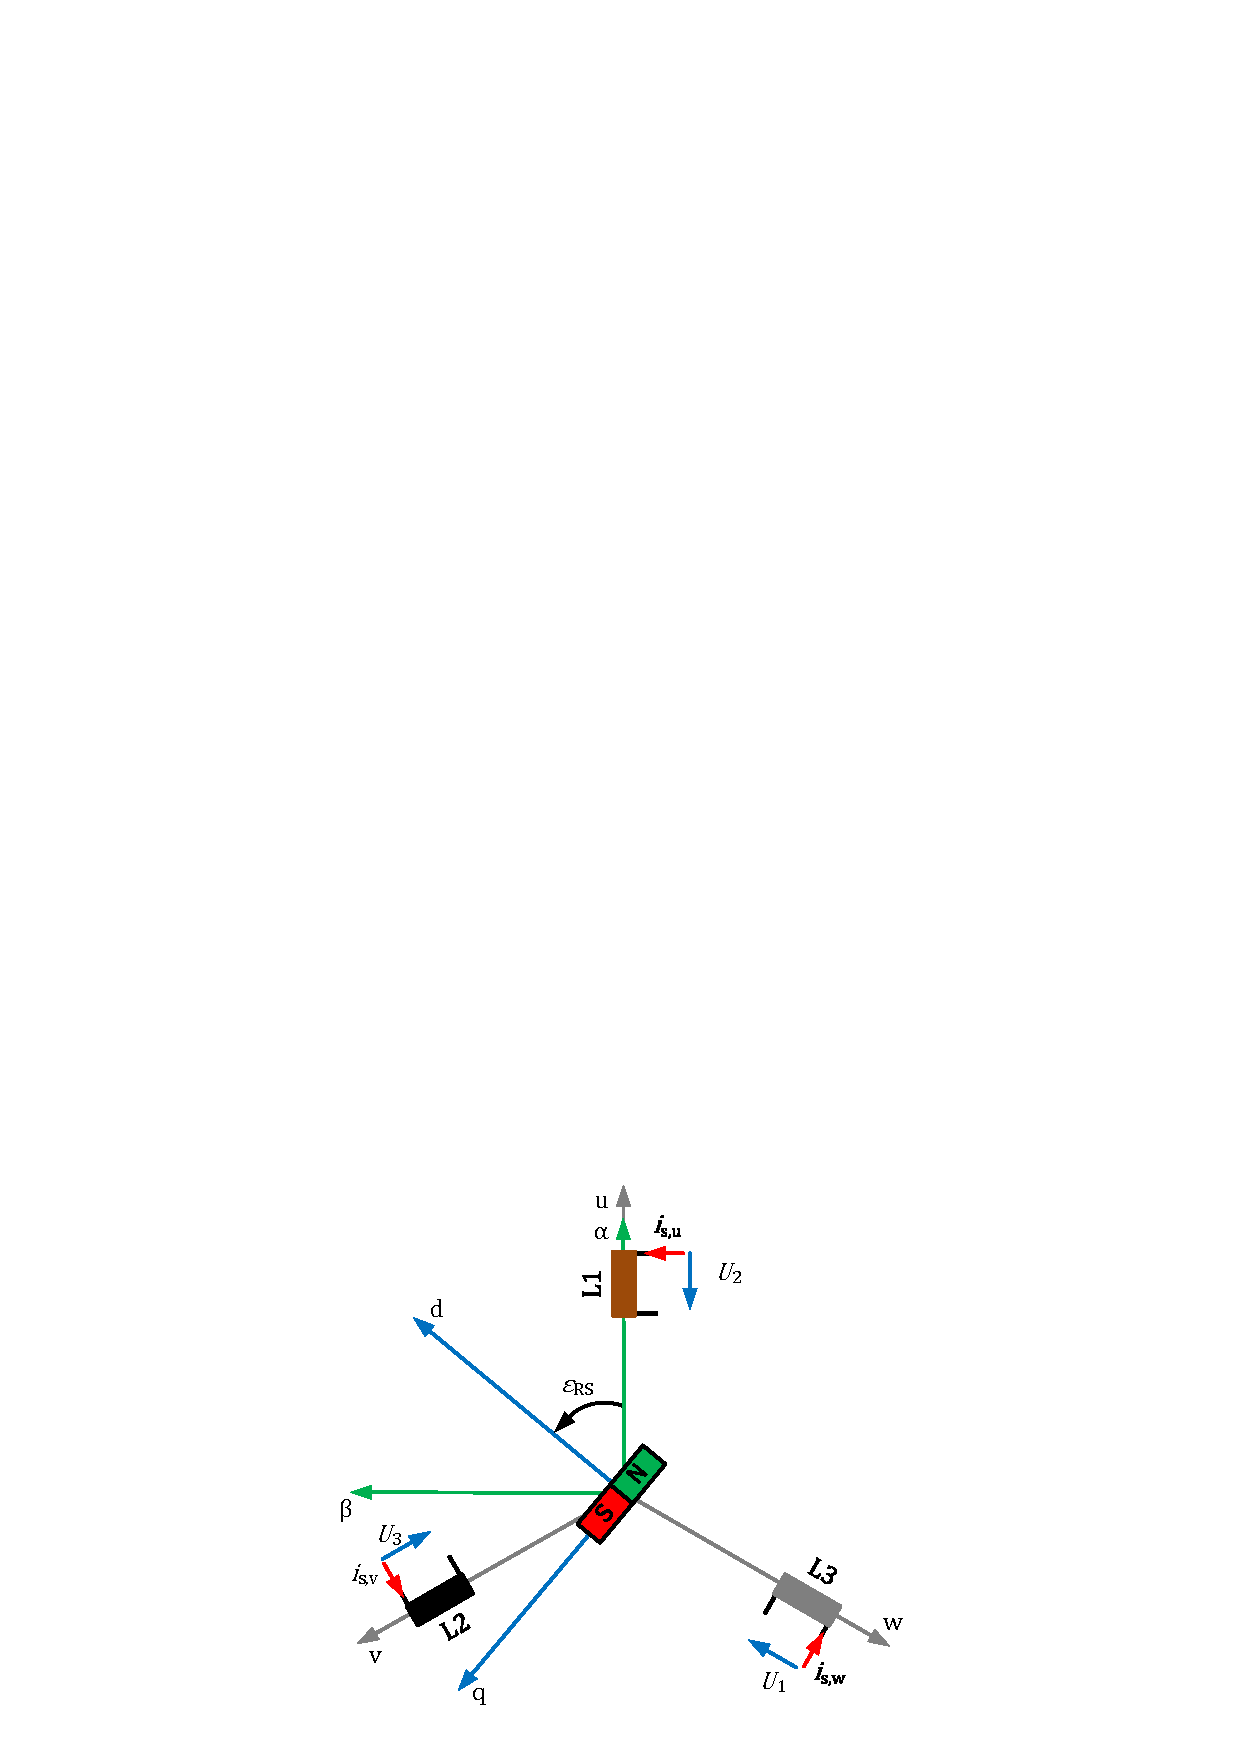
\includegraphics{_Bilder/synchron-grundlage.pdf}
\label{fig:synchron-grundlage}
\caption{Graphische Veranschaulichung der verschiedenen Koordinatensysteme: dreiphasig $(u,
v, w)$, ständerfest $(\alpha, \beta)$ und rotorfest $(d, q)$.}
\end{figure}

Das Induktionsgesetz besagt, dass die in einer Spule induzierte Spannung gleich der entgegengesetzten Änderung der durch die Wicklung der Spule fließenden Flussverkettung ist \autocite{kellner2012}.

\begin{align}
u_\i{q} = - \frac{\i{d}}{\i{d}t}\Psi
\end{align}

\begin{figure}[h!]
\centering
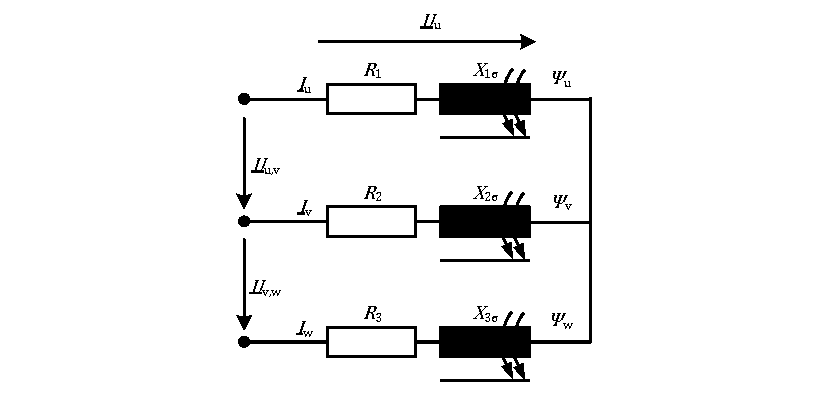
\includegraphics{_Bilder/dq-synchron-rotorfest.pdf}
\label{fig:netzwerk-stander-drehstrom}
\caption{Allgemeines Netzwerk des Ständers einer Drehstrommaschine.}
\end{figure}

Entsprechend Abbildung~\ref{fig:netzwerk-stander-drehstrom} ergeben die die Grundgleichungen einer PMSM ganz allgemein zu

\begin{align}
u_\i{u} = R_\i{1}i_\i{u} + \frac{\i{d}}{\i{d}t}\Psi_\i{u} \nonumber \\ 
u_\i{v} = R_\i{1}i_\i{v} + \frac{\i{d}}{\i{d}t}\Psi_\i{v} \label{eqn:10} \\ 
u_\i{w} = R_\i{1}i_\i{w} + \frac{\i{d}}{\i{d}t}\Psi_\i{w} \nonumber
\end{align}

Es wird im Folgenden davon ausgegangen, dass das dreiphasige System symmetrisch und damit nullsystemfrei ist.
Damit lassen sich komplexe Zahlen zur Darstellung der Ströme und Spannungen verwenden.
Der Komplexe Spannungszeiger in ständerfesten Koordinaten lautet

\begin{align}
\underline{u}^{\alpha, \beta} = \frac{2}{3}(u_\i{u} + \underline{a} u_\i{v} + \underline{a}^2 u_\i{w} ) \quad \text{mit}\,\, \underline{a} = e^{\i{j}2\pi/3} = -\frac{1}{2}+\i{j}\frac{\sqrt{3}}{2} \label{eqn:2}
\end{align}

Eine ausführliche Beschreibung der Raumzeigerdefinition ist in Abschnitt~\ref{sec:raumzeiger} beschrieben.

\begin{quote}
\enquote{Das innere Drehmoment berechnet sich aus den Luftspaltgrößen und enthält daher keine mechanischen Verluste, wie zum Beispiel Reibungsverluste, die in den Motorlagern auftreten.
Bei einer in Sternschaltung betriebenen Maschine, deren Sternpunkt nicht geerdet ist, in Verbindung mit symmetrisch vorgegebenen Klemmenspannungen ist kein Nullsystem vorhanden.
Daher wird zur Vereinfachung der Berechnungen davon ausgegangen, dass das betrachtete System kein Nullsystem besitzt, auch wenn die vom Umrichter erzeugten Spannungen in der Realität nicht ideal sind und die Nullsystemfreiheit nicht für Motoren in Dreiecksschaltung zutrifft \autocite[S.~25]{kellner2012}.}
\end{quote}

Es gilt:

\begin{align}
u_\i{u} + u_\i{v} + u_\i{w} = 0 \label{eqn:3}
\end{align}

Aus den Gleichungen~(\ref{eqn:10}), (\ref{eqn:2}) und (\ref{eqn:3}) ergibt sich dann in ständerfesten Koordinaten abhängig von Phasenströmen und -flussverkettungen

\begin{align}
\underline{u}^{\alpha, \beta} = \frac{2}{3} \left[ (R_\i{1}i_\i{u} + \frac{\i{d}}{\i{d}t}\Psi_\i{u})\cdot (1-\underline{a}^2) + (R_\i{1}i_\i{v} + \frac{\i{d}}{\i{d}t}\Psi_\i{v})\cdot (\underline{a}-\underline{a}^2) \right]
\end{align}

So ergibt sich die Darstellung von Real- und Imaginärteil des Spannungszeigers in ständerfesten Koordinaten nach \textcite{kellner2012} zu:

\begin{align}
	\text{Re}\{ \underline{u}^{\alpha,\beta} \} &= (R_\i{1}i_\i{u}+\frac{\i{d}}{\i{d}t}\Psi_\i{u}) = u_\i{u} \\
	\text{Im}\{ \underline{u}^{\alpha,\beta} \} &= (R_\i{1}i_\i{u}+\frac{\i{d}}{\i{d}t}\Psi_\i{u})\cdot \frac{1}{\sqrt{3}} + (R_\i{1}i_\i{v}+\frac{\i{d}}{\i{d}t}\Psi_\i{v})\cdot \frac{2}{\sqrt{3}} = \frac{u_\i{u}+2u_\i{v}}{\sqrt{3}}
\end{align}

Damit kann die komplexe Spannungsgleichung in $\alpha,\beta$-Koordinaten geschrieben werden:

\begin{align}
	\underline{u}^{\alpha,\beta} = R_\i{1}\cdot\underline{i}^{\alpha,\beta}+\frac{\i{d}}{\i{d}t}\underline{\Psi}^{\alpha,\beta}
\end{align}

mit

\begin{align}
	\underline{i}^{\alpha,\beta} &= i_\i{u} + \underline{a}\cdot i_\i{v} + \underline{a}^{2}\cdot (-i_\i{u}-i_\i{v}) \\
	\underline{\Psi}^{\alpha,\beta} &= \Psi_\i{u} + \underline{a}\cdot \Psi_\i{v} + \underline{a}^{2}\cdot (-\Psi_\i{u}-\Psi_\i{v})
\end{align}

Zusätzlich zum ständerfesten Koordinatensystem kann ein läuferfestes Koordinatensystem eingeführt werden.
Der Vorteil ist, dass die läuferfesten Koordinaten Gleichgrößen sind, während die ständerfesten Koordinaten Wechselgrößen sind.
Die Eigenschaft der läuferfesten Koordinaten wird für die feldorientierte Regelung verwendet \autocites{schroder2001}{nuss2010}{fuest2004}.
Es ist mit den läuferfesten Koordinaten möglich, dass Motormodell entsprechend Gleichung~(\ref{eqn:10}) darzustellen.
Die läuferfesten Koordinaten werden durch Drehung des $\alpha,\beta$-Koordinatensystems um den elektrischen Läuferwinkel $\epsilon_\i{RS}$ gewonnen.
Für einen beispielhaften Zeiger $\underline{\xi}$ gilt nach \textcite{kellner2012}

\begin{align}
	\underline{\xi}^{\alpha,\beta} &= \xi \cdot e^{\x{j}\epsilon_\xi} = \underline{\xi}^{\x{d,q}}\cdot e^{\x{j}\epsilon_\x{el}} \label{eqn:raumzeiger-a-b}\\
	\underline{\xi}^{\x{d,q}} &= \xi \cdot e^{\x{j}(\epsilon_\xi - \epsilon_\x{el})} = \underline{\xi}^{\alpha,\beta} \cdot e^{-\x{j}\epsilon_\x{el}}
\end{align}

Mit Hilfe der Gleichung~(\ref{eqn:raumzeiger-a-b}), lässt sich allgemein der Spannungszeiger umschreiben zu:

\begin{align}
	\underline{u}^{\alpha,\beta} = \underline{u}^{\x{d,q}}\cdot e^{\x{j}\epsilon_\x{el}} = R_\x{1}\underline{i}^{\x{d,q}}\cdot e^{\x{j}\epsilon_\x{el}} + \frac{\x{d}}{\x{d}t}(\underline{\Psi}^{\x{d,q}}e^{\x{j}\epsilon_\x{el}})
\end{align}

Durch Anwendung der Produktregel kann der Fluss umgeschrieben werden.

\begin{align}
	\frac{\x{d}}{\x{d}t}\underline{\Psi}^{\alpha,\beta} &= \frac{\x{d}}{\x{d}t}(\underline{\Psi}^{\x{d,q}}e^{\x{j}\epsilon_\x{el}}) \nonumber \\
														&= e^{\x{j}\epsilon_\x{el}} \cdot \frac{\x{d}}{\x{d}t}\underline{\Psi}^{\x{d,q}} + \underline{\Psi}^{\x{d,q}} \frac{\x{d}}{\x{d}t}e^{\x{j}\epsilon_\x{el}} \\
														&= (\frac{\x{d}}{\x{d}t}\underline{\Psi}^{\x{d,q}}+\x{j}\cdot \omega_\x{el}\underline{\Psi}^{\x{d,q}})e^{\x{j}\epsilon_\x{el}}
\end{align}

Damit ergibt sich der komplexe Zeiger als und vereinfacht Gleichung~(\ref{eqn:udq-zeiger-vereinfacht}):

\begin{align}
	\underline{u}^{\x{d,q}}e^{\x{j}\epsilon_\x{el}} &= R_\x{1}\underline{i}^{\x{d,q}}\cdot e^{\x{j}\epsilon_\x{el}} + (\frac{\x{d}}{\x{d}t}\underline{\Psi}^{\x{d,q}}+\x{j}\cdot \omega_\x{el}\underline{\Psi}^{\x{d,q}})e^{\x{j}\epsilon_\x{el}}\\
	\underline{u}^{\x{d,q}} &= R_\x{1}\underline{i}^{\x{d,q}} + \frac{\x{d}}{\x{d}t}\underline{\Psi}^{\x{d,q}}+\x{j}\cdot \omega_\x{el}\underline{\Psi}^{\x{d,q}}	  \label{eqn:udq-zeiger-vereinfacht}
\end{align}

Die Beziehung (\ref{eqn:udq-zeiger-vereinfacht}) beschreibt den Spannungsraumzeiger in den rotorfesten $d,q$-Koordinaten.
Bei Synchronmaschinen entsprechen die rotorfesten Koordinaten gleichzeitig den flussorientierten Koordinaten, da der Permanentmagnetfluss mit dem Läufer rotiert.
Gleichung~(\ref{eqn:udq-zeiger-vereinfacht}) kann gemäß

\begin{align}
	u_\x{d} + \x{j}u_\x{q} = R_\x{1}(i_\x{d}+\x{j}i_\x{q}) + \frac{\x{d}}{\x{d}t}(\Psi_\x{d}+\x{j}\Psi_\x{q}) + \x{j}\omega_\x{el}(\Psi_\x{d}+\x{j}\Psi_\x{q})
\end{align}

Eine Trennung von Real- und Imaginärteil ergibt die bekannten, üblicherweise verwendeten Gleichungen \autocite{schroder2001}

	\begin{align}
		u_\x{d} &= R_\x{1}i_\x{d} + \frac{\x{d}}{\x{d}t}\Psi_\x{d}-\omega_\x{el}\Psi_\x{q} \label{eqn:ud-gleichung}\\
		u_\x{q} &= R_\x{1}i_\x{q} + \frac{\x{d}}{\x{d}t}\Psi_\x{q}-\omega_\x{el}\Psi_\x{d} \label{eqn:uq-gleichung}
	\end{align}

Allgemein kann das innere Drehmoment einer einpolpaarigen elektrischen Maschine und damit auch im Speziellen einer PMSM nach \textcite{kellner2012} aus dem in Richtung der Motorwelle zeigenden Vektorprodukt aus Ständerfluss und Ständerstrom berechnet werden:

\begin{align}
	M_\x{i} = \frac{3}{2}(\underline{\Psi}^{\x{d,q}} \times \underline{i}^{\x{d,q}}) 
\end{align}

Das innere Drehmoment $M_\x{i}$ für eine elektrische Maschine mit $p\x{p}$ Polpaaren kann schließlich nach Auswertung des Vektorproduktes ermittelt werden:

	\begin{align}
M_\x{i} = \frac{3p}{2} ( \Psi_\x{d}i_\x{q} - \Psi_\x{q}i_\x{d} ) \label{eqn:mi-gleichung}
	\end{align}

Um das System vollständig zu beschreiben, fehlt noch die mechanische Bestimmungsgleichung

\begin{align}
	M_\x{i} - M_\x{Last} = J \frac{\x{d}}{\x{d}t}\omega_\x{mech} = \frac{J}{p\x{p}} \frac{\x{d}}{\x{d}t}\omega_\x{el} \label{eqn:mechanische-gleichung}
\end{align}

Hierbei steht $M_\x{Last}$ für das Lastmoment, $J$ für die Trägheit des Systems und $p\x{p}$ für die Polpaarzahl der elektrischen Maschine.
Alle hergeleiteten Gleichungen beziehen sich auf die Annahme des Grundwellenmodells.
Im nächsten Schritt ist es wichtig, die Flüsse durch Induktivitäten zu ersetzen.
Dafür werden oft linearisierte Gleichungen verwendet \autocite{schroder2001}, bei dem Modell sind alle Parameter konstant.
Dementsprechend einfach ist es, die Ableitungen der Flussverkettungen zu bestimmen.
Beim linearen Maschinenmodell gibt es definitionsgemäß keine Sättigungserscheinungen \autocites{mullerII2008}{schroder2001}.
Alle elektrischen Parameter und damit auch die Induktivitäten der elektrischen Maschine sind damit konstant.
Aus dieser Annahme folgt nach \autocite{schroder2001}:

\begin{align}
	\Psi_\x{d} &= \Psi_{pm} + L_\x{d}i_\x{d} \\
	\Psi_\x{q} &= L_\x{q}i_\x{q}
\end{align}

Die in Richtung der $d$-Achse ausgerichteten Permanentmagnete rufen eine als konstant angenommene Flussverkettung $\Psi_\x{pm}$ hervor \autocite{kellner2012}.
Daraus ergeben sich in Gleichung (\ref{eqn:ud-gleichung}), (\ref{eqn:uq-gleichung}) und (\ref{eqn:mi-gleichung}) eingesetzt die Grundgleichungen des linearisierten Maschinenmodells zu:

\begin{align}
		u_\x{d} &= R_\x{1}i_\x{d} + L_\x{d}\frac{\x{d}i_\x{d}}{\x{d}t}-\omega_\x{el}L_\x{q}i_\x{q} \label{eqn:ud-lin-gleichung} \\
		u_\x{q} &= R_\x{1}i_\x{q} + L_\x{q}\frac{\x{d}i_\x{q}}{\x{d}t}+\omega_\x{el}L_\x{d}i_\x{d} + \omega_\x{el}\Psi_\x{pm}  \label{eqn:uq-lin-gleichung} \\
		M_\x{i} &= \frac{3p}{2} ( \Psi_\x{pm}i_\x{q} + (L_\x{d}-L_\x{q})i_\x{d}i_\x{q}) \label{eqn:mi-lin-gleichung}
\end{align}

\begin{figure}[h!]
	\centering
	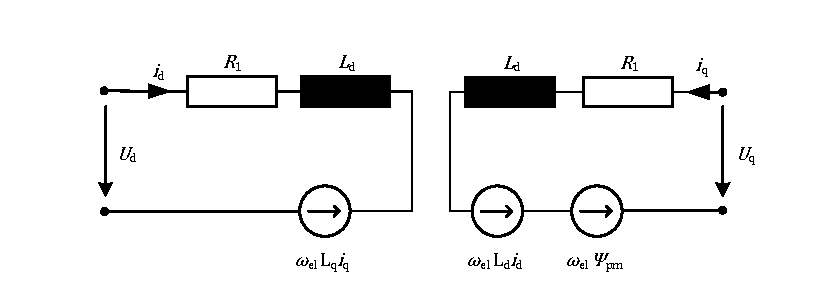
\includegraphics{_Bilder/ESB-synchron-dq.pdf}
	\label{fig:ESB-synchron-dq}
	\caption{Graphische Darstellung der Gleichungen (\ref{eqn:ud-lin-gleichung}) und (\ref{eqn:uq-lin-gleichung}).}
\end{figure}

Die beiden Spannungsgleichungen können gemäß Abbildung \ref{fig:ESB-synchron-dq} graphisch dargestellt werden.
Erkennbar ist, dass in der Abbildung \ref{fig:ESB-synchron-dq} die beiden Gleichungen nur über die Spannungsquellen miteinander verkoppelt sind.
Löst man obenstehende Gleichung mit der mechanischen Gleichung (\ref{eqn:mechanische-gleichung}) nach den Ableitungen von $i_\x{d}, i_\x{q}$ und $\omega_\x{el}$ auf, so ergeben sich die linearen Gleichungen der PMSM in Zustandsform zu:

\begin{align}
\frac{\x{d}i_\x{d}}{\x{d}t} &= -\frac{R_\x{1}}{L_\x{d}}i_\x{d}+\omega_\x{el}\frac{L_\x{q}}{L_\x{d}}i_\x{q}+\frac{1}{L_\x{d}}u_\x{d} \label{eqn:id_dt} \\
\frac{\x{d}i_\x{q}}{\x{d}t} &= -\omega_\x{el}\frac{L_\x{d}}{L_\x{q}}i_\x{d} - \frac{R_\x{1}}{L_\x{q}}i_\x{q} + \frac{1}{L_\x{q}}u_\x{q} - \frac{\omega_\x{el}}{L_\x{q}}\Psi_\x{pm} \label{eqn:iq_dt} \\
\frac{\x{d}\omega_\x{el}}{\x{d}t} &= \frac{3p^2}{2J}(L_\x{d} - L_\x{q})i_\x{q} i_\x{d} + \frac{3p^2}{2J} \Psi_\x{pm} i_\x{q} - \frac{p}{J} M_\x{Last} \label{eqn:dw_dt}
\end{align}

\section{Feldorientierte Regelung}\label{sec:foc}

Die feldorientierte Regelung auch unter \enquote{FOC} bekannt (engl. Field Oriented Control), in Europa als \enquote{vector control} zu finden, ist ein Regelverfahren für Drehstrommaschinen.
In vielen Anwendungen werden Gleichstrommaschinen als Antriebe eingesetzt, da die Einstellmöglichkeiten der Drehzahl in weiten Bereichen auszeichnet.
Drehstromantriebe werden hingegen oft mit einer festen Drehzahl betrieben.
Da die Drehzahl abhängig von der Frequenz der Speisespannung ist, kann eine Drehzahländerung nur durch eine Frequenzänderung des speisenden Netzes geschehen.
Historisch gesehen war dies früher eine große Herausforderung, die mittlerweile durch die Weiterentwicklung der Leistungselektronik einfach zu realisieren ist.
Damit ist man in der Lage Drehstromantriebe mit variabler Drehzahl zu betreiben und verschiedene Arbeitspunkte anzufahren.
Im Gegensatz zu Gleichstrommaschinen besitzen Drehstrommotoren keinen mechanischen Kommutator und damit auch keinem nennenswerten mechanischen Verschleiß.
Zusammen mit der Leistungselektronik lassen sich heute kompakte Antriebe mit einem guten Wirkungsgrad realisieren.
Die feldorientierte Regelung stellt dabei ein geeignetes Verfahren dar, die Synchronmaschine in der Drehzahl zu regeln.

\subsection{Prinzip der FOC}

Das Prinzip der Feldorientierten Regelung beruht auf der Feldorientierung.
Dabei wird ein Koordinatensystem (d,q-Koordinatensystem) auf dem Rotor gelegt, so rotiert das Koordinatensystem mit dem Rotor und dem magnetischen Feld.
Somit lassen sich die gleichen Gleichungen wie bei der Gleichstrommaschine verwenden (s.~h.~Abb.~\ref{fig:foc-dc-ac}).

\begin{figure}[h!]
	\centering
	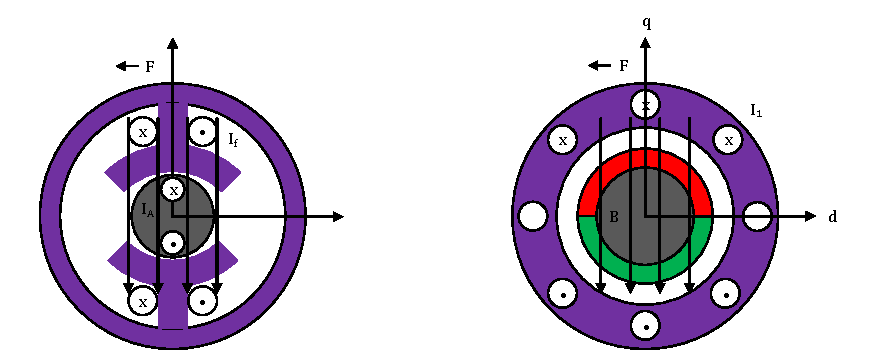
\includegraphics{_Bilder/foc-dc-ac.pdf}
	\label{fig:foc-dc-ac}
	\caption{Veranschaulichung der Feldorientierten Regelung im Vergleich mit einer DC-Maschine.}
\end{figure}

Gleichung~(\ref{eqn:mi-gleichung}) beschreibt das Drehmoment der elektrischen Maschine als Ergebnis des Kreuzproduktes zwischen Ständerflussverkettung und Ständerstrom.
Das Drehmoment der Maschine ist daher genau dann optimal, wenn Statorfluss und Statorstrom orthogonal zueinander stehen.
Ist die Lage des Statorflusses bekannt, kann der Stromzeiger orthogonal dazu eingestellt werden.
Das Drehmoment der Maschine ist dann nur noch von der Amplitude des Statorstromes abhängig.
Aus reglungstechnisches Sicht kann die feldorientiert geregelte Synchronmaschine mit der Gleichstrommaschine verglichen werden \autocite{Thur2006}.
Wird der Fluss in der Statorwicklung durch Sensoren ermittelt, spricht man von direkter Feldorientierung.
Diese Methode ist sehr präzise, in der Praxis ist sie jedoch nur mit Sondermaschinen realisierbar \autocite{Thur2006}.
Im Allgemeinen wird der Ständerfluss durch ein Modell wie bspw.\ die Integration der Ständerspannung ermittelt.
Die unterschiedlichen Konzepte zur Feldorientierung unterscheiden sich genau in diesem Modell.
Alle diese Methoden werden als indirekte Feldorientierung bezeichnet \autocite{Thur2006}.

\begin{landscape}
\subsection{Beispiel einer FOC bei einer PMSM}
\begin{figure}[h!]
%	\centering
	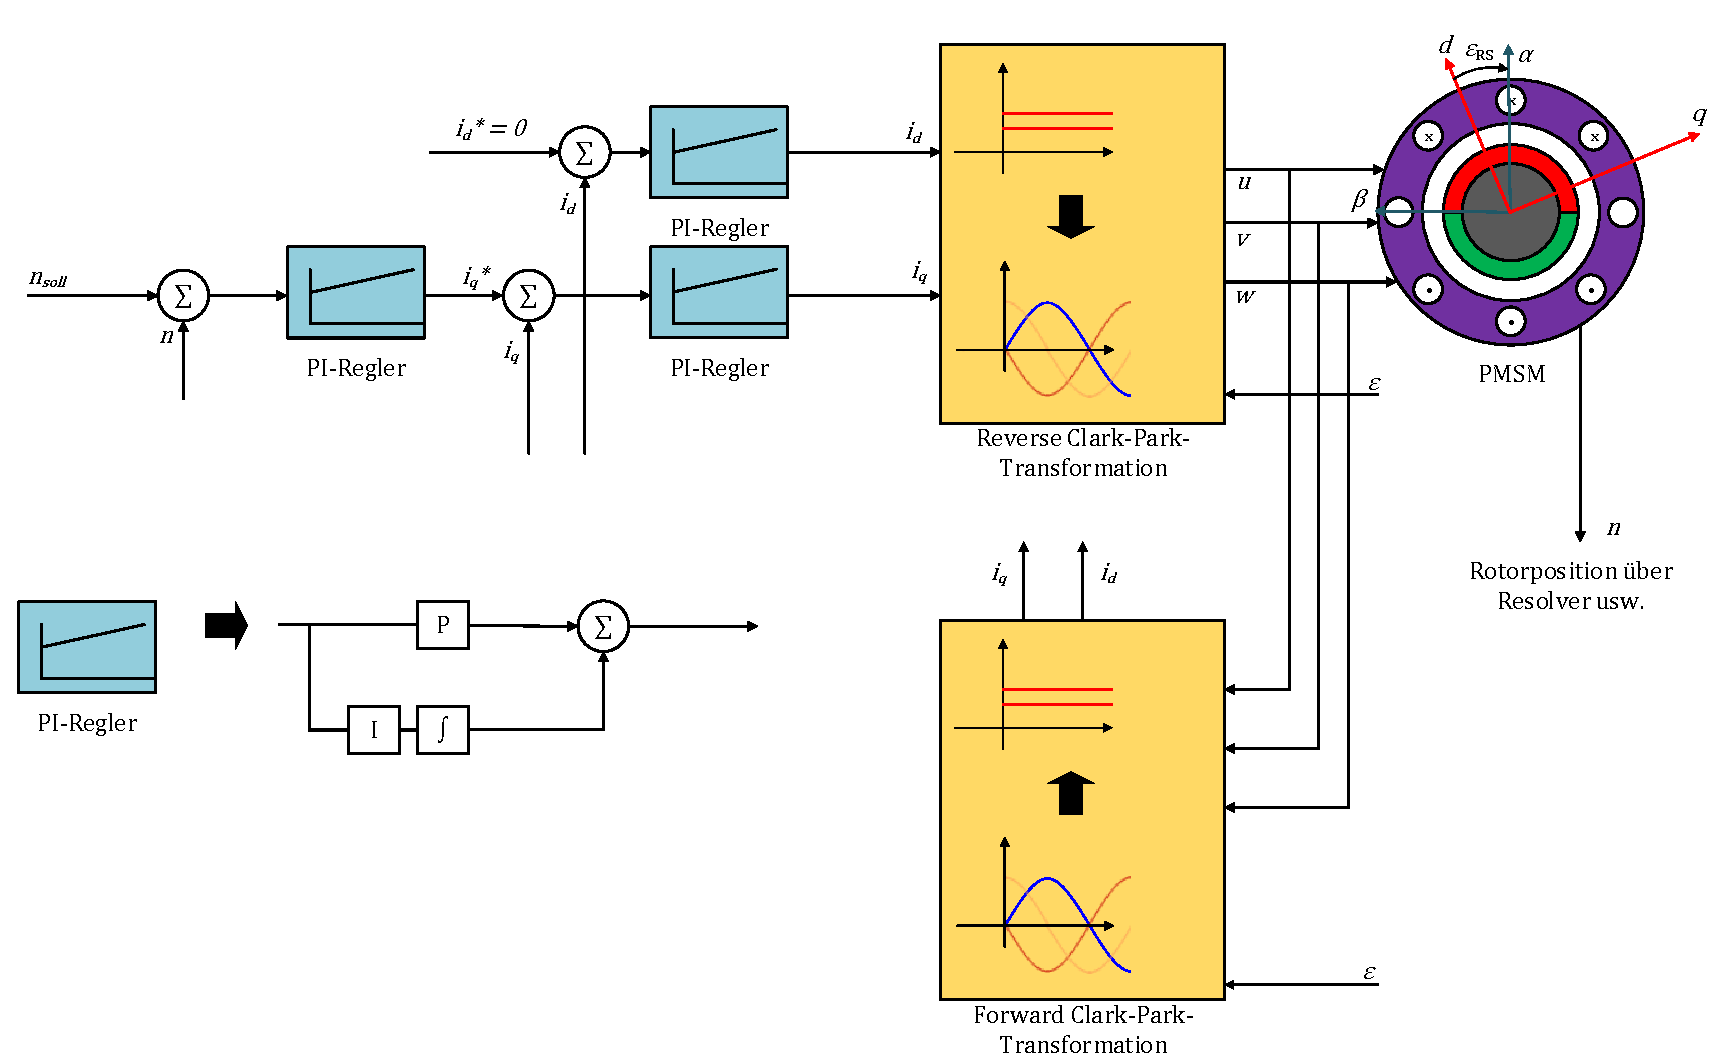
\includegraphics[scale=0.7]{_Bilder/blockschaltbild-foc.pdf}
	\label{fig:foc-dc-ac}
	\caption{Blockschaltbild der Feldorientierten Regelung anhand einer PMSM.}
\end{figure}
\end{landscape}
%%% Local Variables: 
%%% mode: latex
%%% TeX-master: "main.tex"
%%% TeX-open-quote: "\\enquote{"
%%% TeX-close-quote: "}"
%%% LaTeX-csquotes-open-quote: "\\enquote{"
%%% LaTeX-csquotes-close-quote: "}"
%%% End: 

